% Created 2023-09-11 Mo 20:11
% Intended LaTeX compiler: pdflatex
\documentclass[11pt]{article}
\usepackage[utf8]{inputenc}
\usepackage[T1]{fontenc}
\usepackage{graphicx}
\usepackage{grffile}
\usepackage{longtable}
\usepackage{wrapfig}
\usepackage{rotating}
\usepackage[normalem]{ulem}
\usepackage{amsmath}
\usepackage{textcomp}
\usepackage{amssymb}
\usepackage{capt-of}
\usepackage{hyperref}
\author{Marcel Schaible}
\date{\today}
\title{Wasserspeicher}
\hypersetup{
 pdfauthor={Marcel Schaible},
 pdftitle={Wasserspeicher},
 pdfkeywords={},
 pdfsubject={},
 pdfcreator={Emacs 27.2 (Org mode 9.4.4)}, 
 pdflang={Germanb}}
\begin{document}

\maketitle
\tableofcontents


\section{Wasserspeicher}
\label{sec:org89e9aa8}



\href{./wasserSpeicher.pdf}{Wasserspeicher}\\

\begin{itemize}
\item Wassertank\\
\item Aktoren:\\
1x Pumpe, Drehzahlgesteuert\\
1x Ventil, Offen/Geschlossen\\
2x Drucksensoren\\
\item Verbraucher\\
\end{itemize}

\href{https://www.leifiphysik.de/mechanik/druck-und-auftrieb/grundwissen/schweredruck}{Schweredruck am Boden einer Wassersäule}\\

Es sei ein Wassertank mit folgenden Abmessungen gegeben\\

\begin{center}
\begin{tabular}{ll}
Länge & 5m\\
Breite & 2m\\
Höhe & 3m\\
\end{tabular}
\end{center}

Der Druck ist allgemein definiert als Kraft pro Fläche\\
\(p =\frac{F_G}{A}\)\\



Damit sind Echtzeitsysteme digitale Datenverarbeitungsanlagen bei\\
denen der Nutzen eines Berechnungsergebnisses nicht nur vom Ergebnis\\
selbst, sondern auch vom Zeitpunkt der Auslieferung abhängt.\\

Als Beispiel für eine typische Prozessautomatisierung ist In Abbildung\\
\ref{fig:pumpstation} eine schematische Darstellung einer Pumpstation\\
mit folgenden Komponenten dargestellt:\\

\begin{itemize}
    \item Pumpe
    \item Manometer
    \item Stellventil
    \item Reservoir
\end{itemize}

F"ur einen Wasserturm, vom dem fortw"ahrend Verbraucher alleine durch\\
die Schwerkraft Wasser entnehmen k"onnen, zu betreiben muss das Reservoir\\
stets hinreichend\\
gef"ullt sein. Wenn der Wasserstand unter der \textit{leer} Marke ist\\
dann muss die Pumpe gestartet werde.\\
Um die Pumpe einzuschalten muss zuerst der Pumpenmotor über das\\
Steuersignal \textit{ein/aus} eingeschaltet werden.  Die Spezifikation\\
der Pumpe bestimmt das Zeitdauer bis ein vorher festgelegter Druck am\\
Ventil anliegt.  Dieser Druck kann mittels des Manometers\\
kontinuierlich am Signal \textit{Druck} gemessen werden.  Falls der\\
gemessene Druck niedriger als der Solldruck ist, kann unter\\
Zuhilfenahme des Drehzahlgebers überprüft werden ob  die Pumpe defekt ist\\
oder keine Flüssigkeit in der Leitung zur Verfügung steht.\\
Erreicht der Druck den Solldruck wird das Ventil durch\\
einschalten des Stellmotors (Signale \textit{oeffnen} und \textit{schliessen})\\
geöffnet. Damit wird unzul"assiger ein R"uckflu"s aus dem Reservoir in das\\
prim"are  Versorgungsnetz vermieden.\\
Dies benötigt je nach Bauweise\\
des Ventils eine genau definierte Zeit.  Der Ventilstatus kann durch\\
die Signale \textit{offen} und \textit{zu} kontrolliert werden.\\
Um den Pumpprozess zu beenden muss zuerst das Ventil geschlossen werden.\\
Dies kann wiederum über den Ventilstatus abgefragt werden.\\
Danach kann der Pumpenmotor ausgeschaltet werden.\\

\begin{figure}[htbp]
\centering
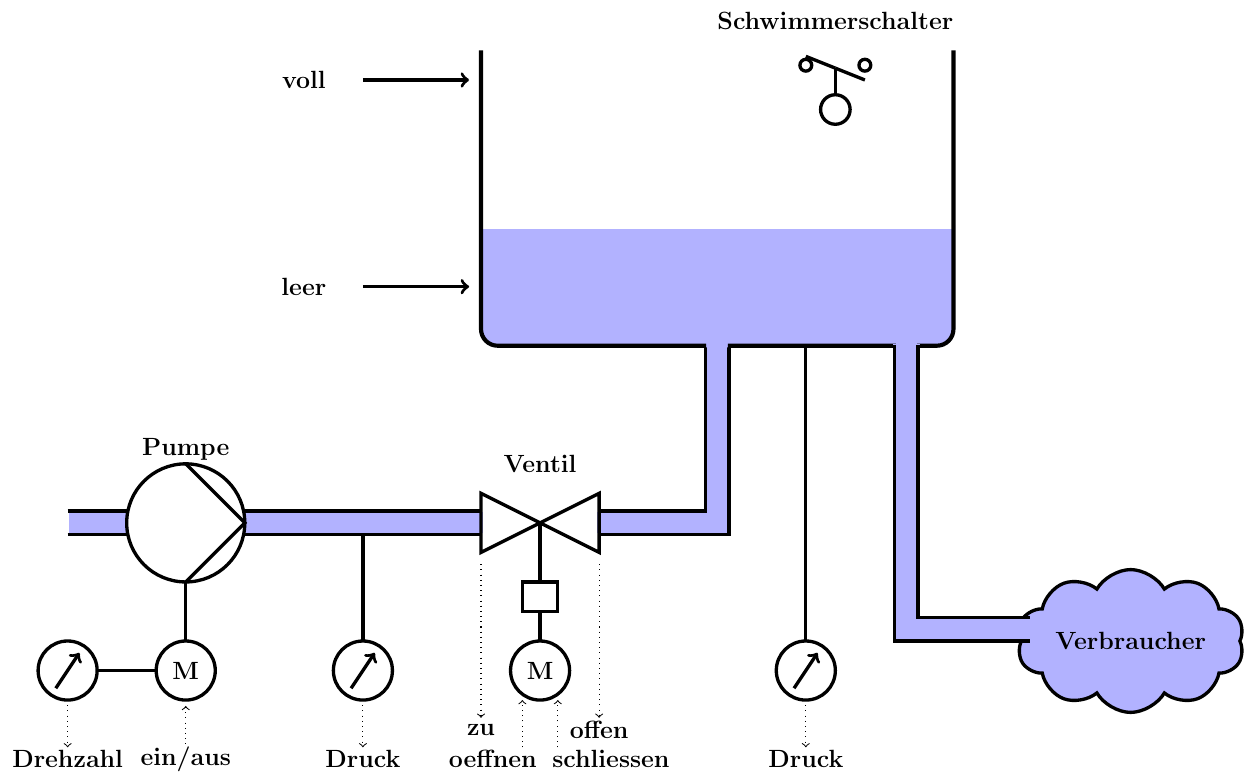
\includegraphics[width=.9\linewidth]{./wasserspeicher.png}
\caption{\label{fig:orga79ebf5}Wasserspeicher}
\end{figure}

\begin{figure}[!htbp]
\centering
  % Requires \usepackage{graphicx}
  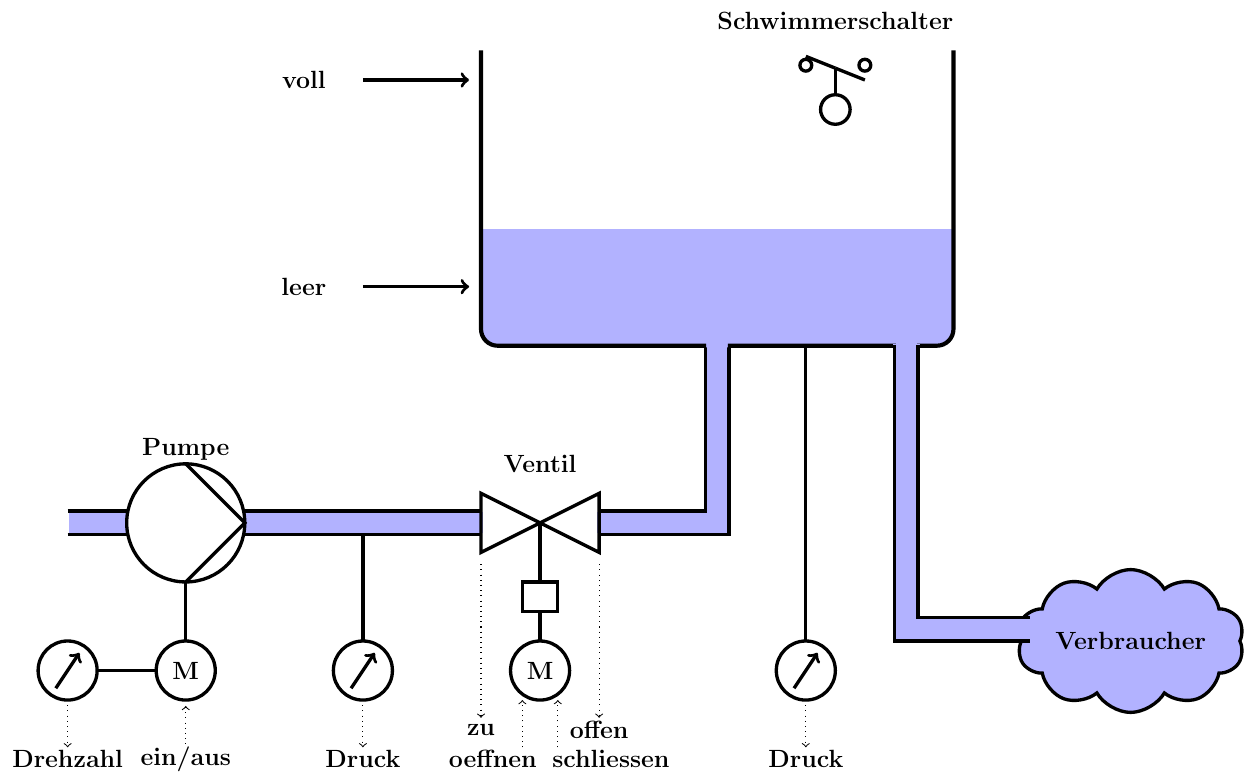
\includegraphics[width=1.0\textwidth]{wasserspeicher.png}\\
   \caption{Wasserspeicher}
  \label{fig:Wasserspeicher}
\end{figure}


\begin{verbatim}
tail -f --follow=name --retry sim.log
\end{verbatim}


 \begin{table}[h!]
\begin{tabular}{p{20pt} p{20pt} p{20pt} p{20pt} p{20pt} p{20pt} p{20pt} p{20pt} p{20pt} p{20pt} p{20pt} p{20pt} p{20pt} p{20pt} p{20pt}  >{\centering\arraybackslash}m{20pt}}
\centering 15 & \centering 14 & \centering 13 & \centering 12 & \centering 11 & \centering 10 & \centering 9 & \centering 8 & \centering 7 & \centering 6 & \centering 5 & \centering 4 & \centering 3 & \centering 2 & \centering 1 & 0\\\hline
\multicolumn{1}{|c|}{Sim} & 
\multicolumn{1}{c|}{Pump} & 
\multicolumn{1}{c|}{Pump rpm} & 
\multicolumn{5}{|c|}{\cellcolor{gray!25}} & 
\multicolumn{1}{c|}{DIR} & 
\multicolumn{7}{c|}{PWM} \\\hline
\end{tabular}
\end{table}

\begin{quote}
simulation\_is\_running,\\
pump\_enabled,\\
pump\_current\_rpm\\
pressure\_sensor\_1\\
valve\_enabled\\
pressure\_sensor\_2\\
current\_consumer\_dissipation\\
\end{quote}

\begin{note}
This is a useful note.\\
\end{note}



\begin{verbatim}
12:00:01.157 SIM: |1|1| 500|    0.0000|0|    0.0000|    0.0000|
\end{verbatim}
\end{document}